\documentclass[a4paper, 12pt]{article}

\usepackage{cmap}
\usepackage{mathtext} 
\usepackage[T2A]{fontenc}
\usepackage[utf8]{inputenc}
\usepackage[english,russian]{babel}	

\usepackage{amsfonts,amssymb,amsthm,mathtools}
\usepackage{amsmath}
\usepackage{icomma} 
\usepackage{float}

\usepackage{graphicx} 
\graphicspath{{Picturies/}}
\usepackage{wrapfig}

\usepackage{array,tabularx,tabulary,booktabs}
\usepackage{longtable}
\usepackage{multirow}

\usepackage{caption}
\captionsetup{labelsep=period}

\renewcommand{\phi}{\varphi}
\newcommand{\eps}{\varepsilon}
\renewcommand{\AA}{\ensuremath{\mathring{A}}}
\newcommand{\parag}[1]{\paragraph*{#1:}}

\newcounter{Points}
\setcounter{Points}{1}
\newcommand{\point}{\arabic{Points}. \addtocounter{Points}{1}}

\author{Калинин Даниил, Б01-108}
\date{\today}
\title{Лабораторная работа 5.1.1. Экспериментальная проверка уравнения Эйнштейна для фотоэффекта и определение постоянной Планка.}

\begin{document}
\maketitle
\parindent=0cm

\parag {Цель работы }
Исследовать зависимость фототока от величины задерживающего потенциала и частоты падающего излучения, что позволяет вычислить величину постоянной Планка.


\parag {Теоритическая справка} ~\\

Фотоэффект --- явление испускания электронов фотокатодом, облучаемым светом,  Это явление хорошо объясняется фотонной теорией света. Взаимодействие монохроматического света с веществом можно описывать
как взаимодействие с веществом частиц, называемых фотонами, которые обладают энергией $ \hbar \omega $ и импульсом $ \hbar\omega/c $. При столкновении фотона с электроном фотокатода энергия фотона полностью передается электрону, и фотон прекращает свое существование. Энергетический баланс этого взаимодействия для вылетающих электронов
описывается уравнением

\begin{equation}\label{energy balance}
\hbar \omega = E_{max} + W
\end{equation}

\begin{figure}[H]
    \centering
    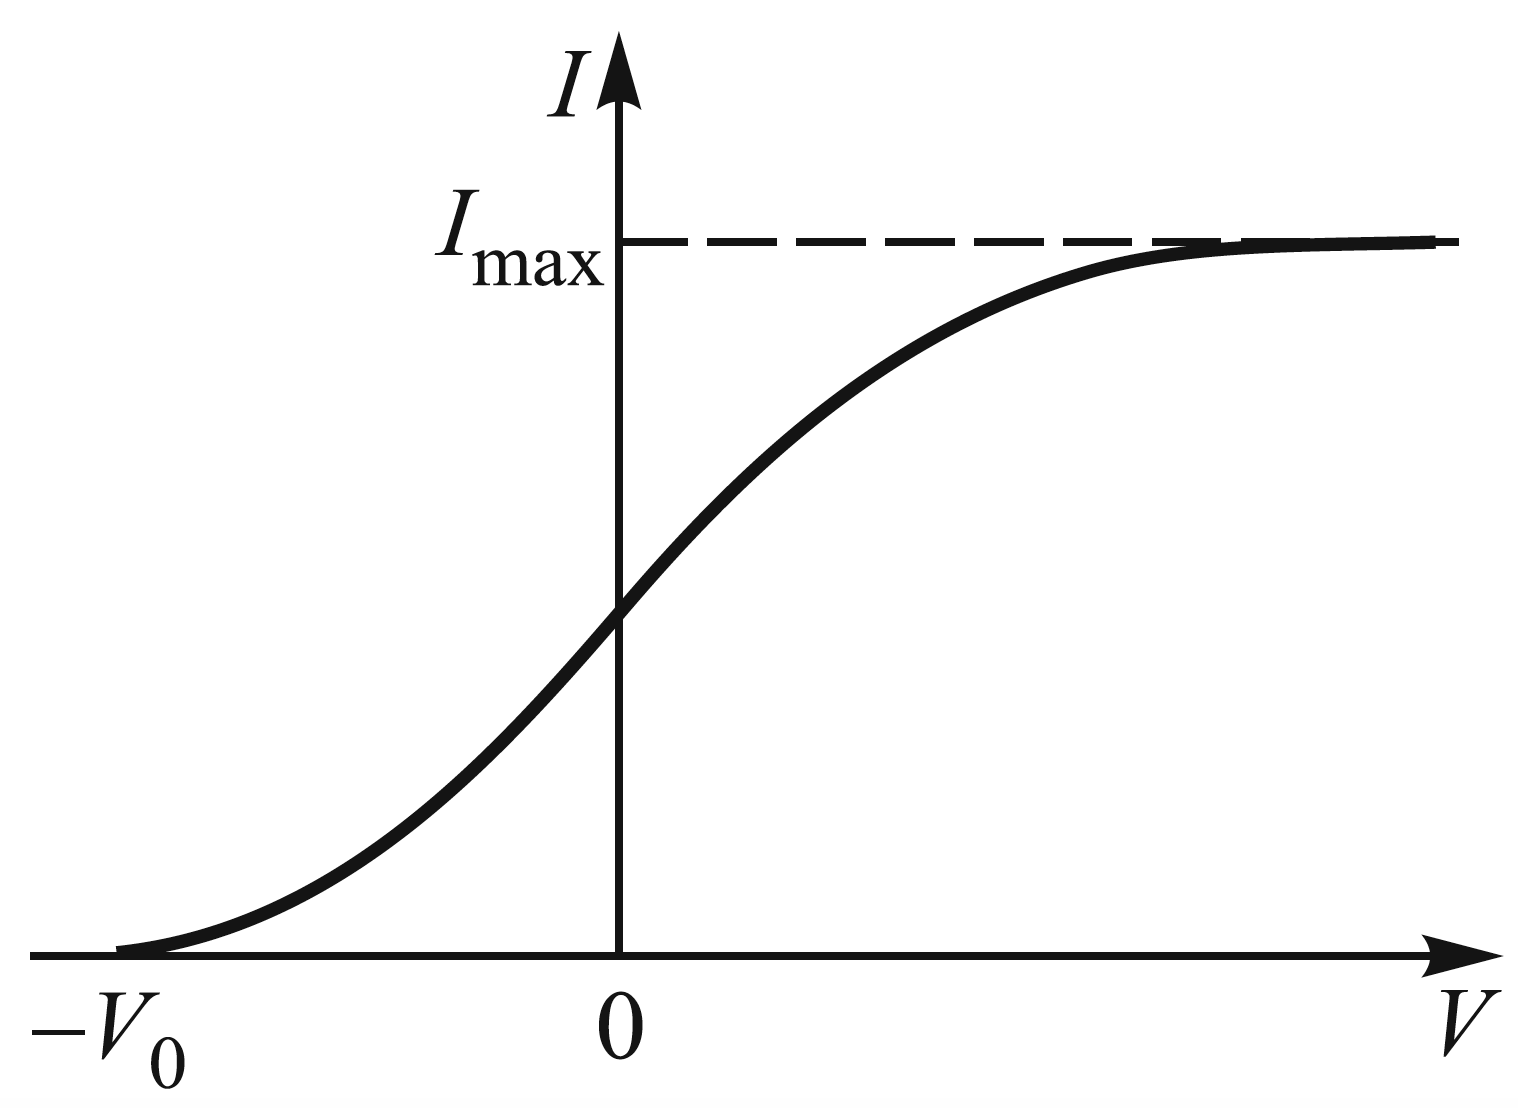
\includegraphics[scale=0.3]{I(V)}
    \caption{Зависимость фототока от напряжения на аноде фотоэлемента}
    \label{ris I(V)}
\end{figure}

Здесь $ E_{max} $ ---  максимальная кинетическая энергия электрона после выхода из фотокатода, $ W $ --- работа выхода электрона из катода. Реально энергетический спектр вылетевших из фотокатода электронов непрерывен --- он простирается от нуля до $ E_{max} $. 

Для измерения энергии вылетевших фотоэлектронов вблизи фотокатода
обычно располагается второй электрод
(анод), на который подается задерживающий ($ V < 0 $) или ускоряющий ($ V >
0 $) потенциал. При достаточно больших
ускоряющих напряжениях фототок достигает насыщения (рис. \ref{ris I(V)}): все испущенные электроны попадают на анод.

При задерживающих потенциалах на анод попадают лишь электроны,
обладающие достаточно большой кинетической энергией, в то время
как медленно движущиеся электроны заворачиваются полем и возвращаются на катод. При некотором значении $ V = -V_0 $ (потенциал запирания) даже наиболее быстрые фотоэлектроны не могут достичь
анода.
Максимальная кинетическая энергия $ E_{max} $ электронов связана с
запирающим потенциалом $ V_0 $ очевидным соотношением $ E_{max} = eV_0 $. Тогда \eqref{energy balance} примет вид, называемый уравнением Эйнштейна:

\begin{equation}\label{Einsteain}
    eV_0 = \hbar\omega - W 
\end{equation}

Чтобы определить величину запирающего
напряжения, нам надо правильно экстраполировать получаемую токовую зависимость к нулю, т. е. определить, какова функциональная
зависимость $ I(V) $. Расчет для простейшей геометрии --- плоский катод, освещаемый светом, и параллельный ему анод --- приводит к зависимости

\begin{equation}\label{sqrt I = V}
    \sqrt{I} \propto V_0 - V
\end{equation}

т. е. корень квадратный из фототока линейно
зависит от запирающего напряжения. Эта зависимость хорошо описывает экспериментальные данные.

В работе изучается зависимость фототока из фотоэлемента от величины задерживающего потенциала $ V $ для различных частот света $ \omega $, лежащих в видимой области спектра. С целью экспериментальной
проверки уравнения Эйнштейна определяются потенциалы запирания
$ V_0 $ при разных частотах света и строится зависимость $ V_0(\omega) $, которая, как это следует из \eqref{Einsteain}, должна иметь вид

\begin{equation}\label{V(w)}
V_0 (\omega) = \dfrac{\hbar\omega - W}{e}
\end{equation}

\begin{figure}[H]
    \centering
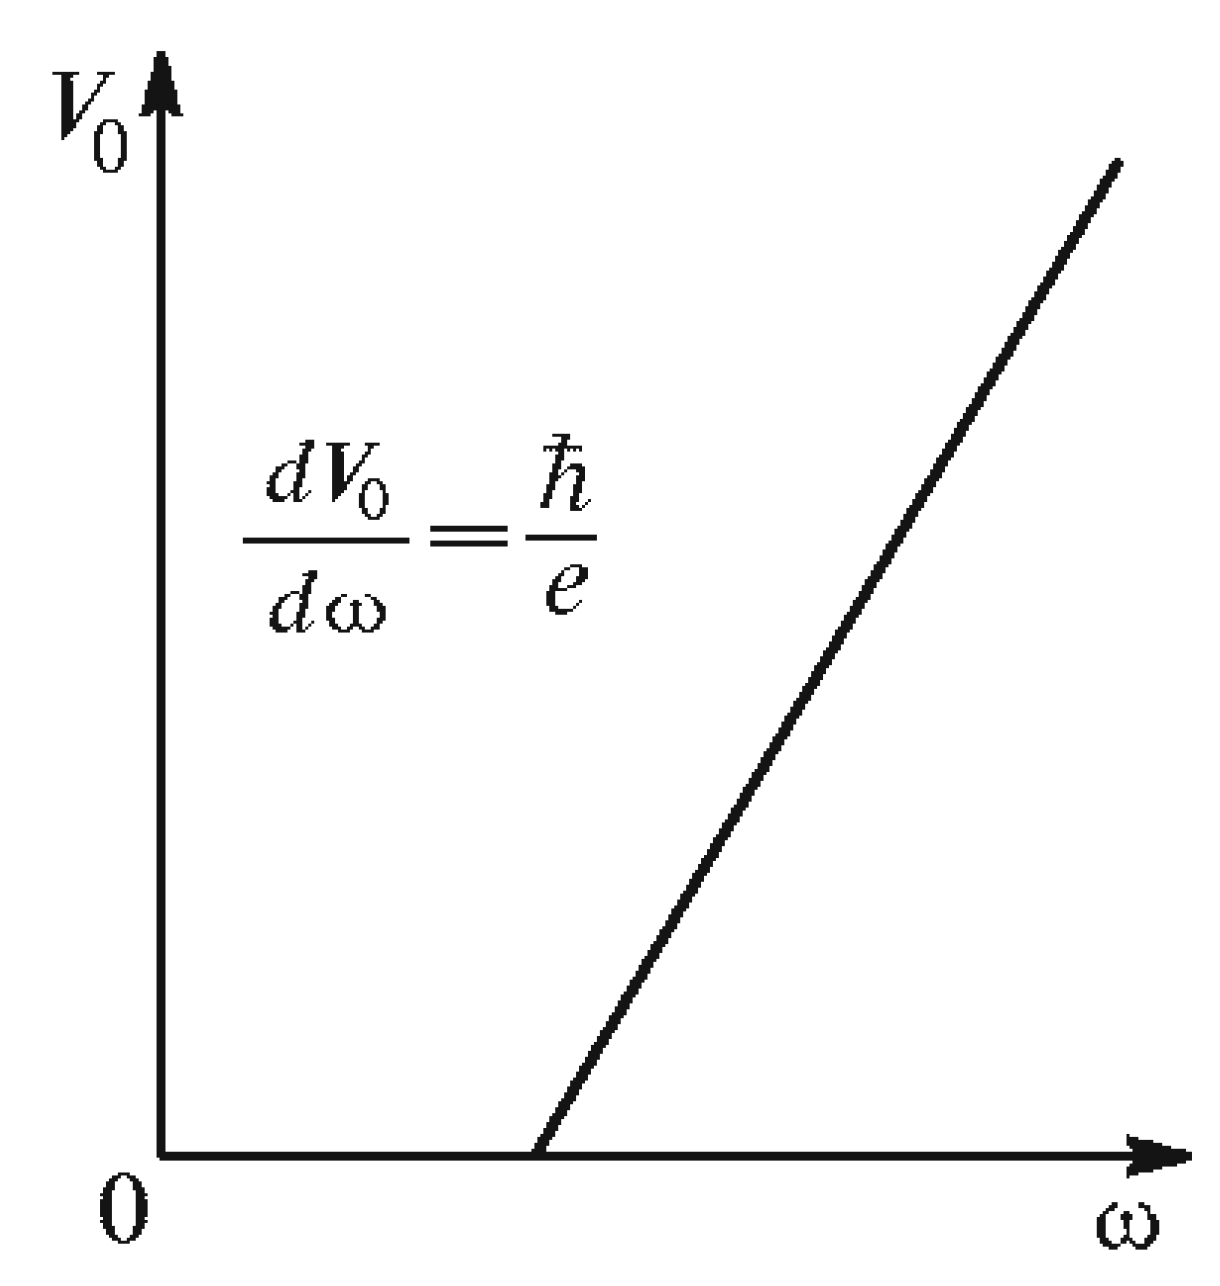
\includegraphics[scale=0.3]{V(w)}
    \caption{Зависимость запирающего потенциала
        от частоты света}
    \label{ris V(w)}
\end{figure}

Потенциал запирания $ V_0 $ для любого катода линейно зависит от
частоты света $ \omega $. По наклону прямой на графике $ V_0(\omega) $ (рис. \ref{ris V(w)}) можно определить постоянную Планка:

\begin{equation}\label{dV/dw}
\dfrac{dV_0}{d\omega} = \dfrac{\hbar}{e}
\end{equation}

Как показывает формула \eqref{dV/dw}, угол наклона прямой $ V_0(\omega) $ не зависит от рода вещества, из которого изготовлен фотокатод. От рода вещества, однако, зависит величина фототока, работа выхода $ W $ и форма кривой $ I(V) $ (рис. \ref{ris I(V)}). Все это определяет выбор пригодных для
опыта катодов.

\parag {Экспериментальная установка}~\\

На рис. \ref{img:work} изображена схема установки. На ней:

\begin{itemize}
    \item 1 --- входная щель.
    \item 2 --- коллиматорный объектив.
    \item 3 --- сложная спектральная призма, склеенная из $П_1$, $П_2$ и $П_3$.
    \item 4 --- объектив зрительной трубы.
    \item 5 --- окуляр зрительной трубы.
    \item 6 --- поворотный столик для 3.
    \item 7 --- микрометрический винт с отсчётным барабаном для 6.
    \item 8 --- микрометрический винт для 2.
    \item 9 --- микрометрический винт для 1.
    \item 10 --- острие указателя.
    \item 11 --- массивный корпус, спасающий установку от студентов.
    \item Л --- источник света.
    \item К --- конденсор (для концентрации света на входной щели).
    \item Оптическая скамья --- нужна для размещения Л и К.
    \item Пульт управления.
\end{itemize}

\begin{figure}[H]
    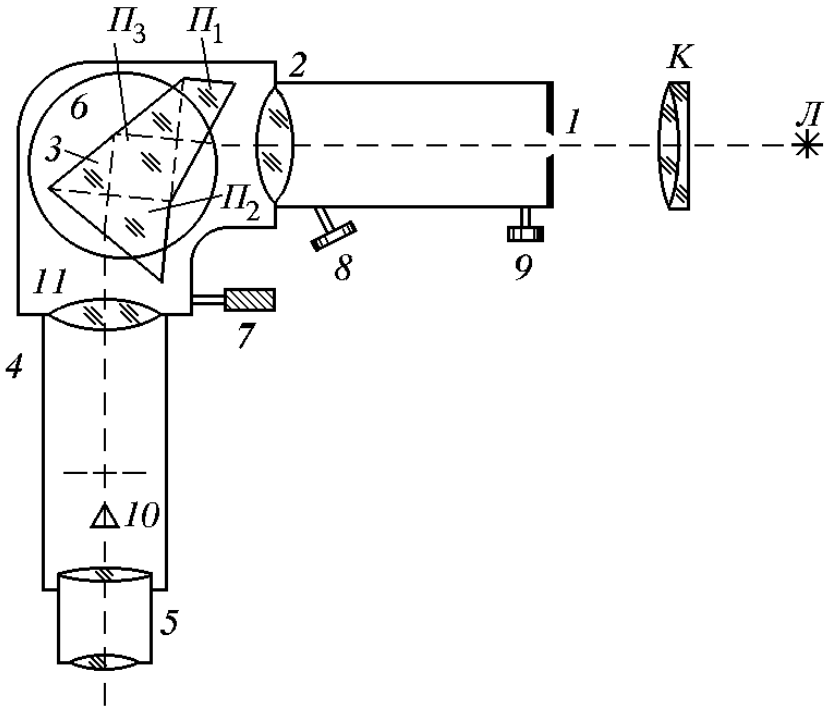
\includegraphics[scale = 0.4]{Workplace}
    \centering
    \caption{Схема экспериментальной установки}
    \label{img:work}
\end{figure}

\parag {Ход работы} ~\\

\point Ознакомимся с принципом работы установки. Включим её и неоновую лампу в сеть, отцентруем её по высоте. Конденсор расположим в 25 см от щели. Настроимся на резкое изображение кончика указателя, вращая глазную линзу окуляра. Отрегулируем яркость освещения указателя с помощью реостата.

\point Вращая барабан, настроимся на жёлтую линию неона (она одна из самых ярких). Перемещая коллиматор винтом 8, получим резкое изображение.

\point Найдём нуль микрометрического винта. Получаем: $0.13$ мм. Установим ширину $0.2$ мм.

\point Закончим насторйку окуляра. Для этого сделаем резкость такой, чтобы параллакс (т.е. смещение указателя относительно линии при движении глаза) отсутствовал.

\point Теперь проведём градуировку спектрометра по спектрам неона. Для этого запишем расположение их спектральных линий на барабане и соответствующие им табличные значения длин волн. Результаты представлены в таблице \ref{tab:neon}.

\point Составим градуировочную кривую с помощью линий спектра неона и ртути. Исходя из предположения, что эта кривая задаётся формулой вида:

\[
    \lambda = a e^{b \phi} + c
\]

Найдём коэффициенты $a$, $b$ и $c$ с помощью МНК. Результаты представлены на рис. \ref {img:calib}:

\begin{align*}
    a &= (201 \pm 7) \AA \\
    b &= (1.05 \pm 0.01) \cdot 10^{-3} \\
    c &= (3960 \pm 20) \AA \\
\end{align*}

\point Теперь проведем 7 серий измерений зависимости фототока от напряжения для разных длин волн падающего света, изменяя на монохроматоре параметр $\phi$ и переводя его в длину волны с помощью градуировки. Ток приведен в безразмерных единицах в силу работы установки. 
	
Результаты измерений сведем в таблицы. Для первой выбранной длины волны ($\phi = 1880^\circ, \lambda = 5402 \AA$) проведем измерения во всем спектре возможных напряжений, а для остальных --- лишь при достаточно малых значениях тока и напряжения (т.е. вблизи потенциала запирания, где искомая зависимость описывается формулой \eqref{sqrt I = V}). Согласно этой формуле, построим графики зависимости в координатах $ \sqrt{I} (V) $ и аппроксимируем линейные участки прямой. Экстраполируя прямую к нулю, получим значения потенциала запирания для каждой серии измерения (длины волны). Результаты сведем в таблицу. 

\point Теперь найдём по графикам запирающее напряжение $V_0$ и построим график $V_0(\omega)$.

Из графика получаем, что:

\[
    \frac{dV_0}{d\omega} = (6.2 \pm 0.4) \cdot 10^{-16} \rightarrow \hbar = (0.99 \pm 0.06) \cdot 10^{-34} ~Дж \cdot с
\]

Что в рамках погрешности согласуется с табличным значением $\hbar = 1.054 \cdot 10^{-34} ~Дж \cdot с$.

\point Найдём красную границу спектра, получаем $\omega_к = (1.56 \pm 0.12) \cdot 10^{15} Гц$

\point Найдём работу выхода как $W = \hbar \cdot \omega_к = (2.40 \pm 0.18) \cdot 10^{-19} Дж = (1.50 \pm 0.12) эВ$

\parag {Заключение} ~\\
Таким образом, в ходе выполнения работы мы проверили Энштейновское описание фотоэффекта и с помощью уравнения последнего измерили постоянную Планка. Результаты вполне согласуются с табличными.

\begin{table}[H]
    \centering
    \begin{tabular}{|c|c|c|c|c|c|c|c|c|c|}
        \hline
        n & 1 & 2 & 3 & 4 & 5 & 6 & 7 & 8 & 9 \\ \hline
        $\lambda$, $\AA$ & 7032 & 6929 & 6717 & 6678 & 6599 & 6533 & 6507 & 6402 & 6383 \\ \hline
        $\phi$, $~^\circ$ & 2600 & 2568 & 2498 & 2486 & 2458 & 2434 & 2422 & 2384 & 2376 \\ \hline
    \end{tabular}
    \\~\\
    \begin{tabular}{|c|c|c|c|c|c|c|c|c|}
        \hline
        n & 10 & 11 & 12 & 13 & 14 & 15 & 16 & 17 \\ \hline
        $\lambda$, $\AA$ & 6334 & 6305 & 6267 & 6217 & 6164 & 6143 & 6096 & 6074 \\ \hline
        $\phi$, $~^\circ$ & 2356 & 2344 & 2328 & 2306 & 2286 & 2274 & 2254 & 2244 \\ \hline
    \end{tabular}
    \\~\\
    \begin{tabular}{|c|c|c|c|c|c|c|c|c|}
        \hline
        n & 18 & 19 & 20 & 21 & 22 & 23 & 24 & 25 \\ \hline
        $\lambda$, $\AA$ & 6030 & 5976 & 5945 & 5882 & 5852 & 5401 & 5341 & 5331 \\ \hline
        $\phi$, $~^\circ$ & 2224 & 2200 & 2184 & 2152 & 2138 & 1880 & 1840 & 1832
        \\ \hline
    \end{tabular}
    \caption {Спектр неона.}
    \label{tab:neon}
\end{table}

\begin{figure}[H]
    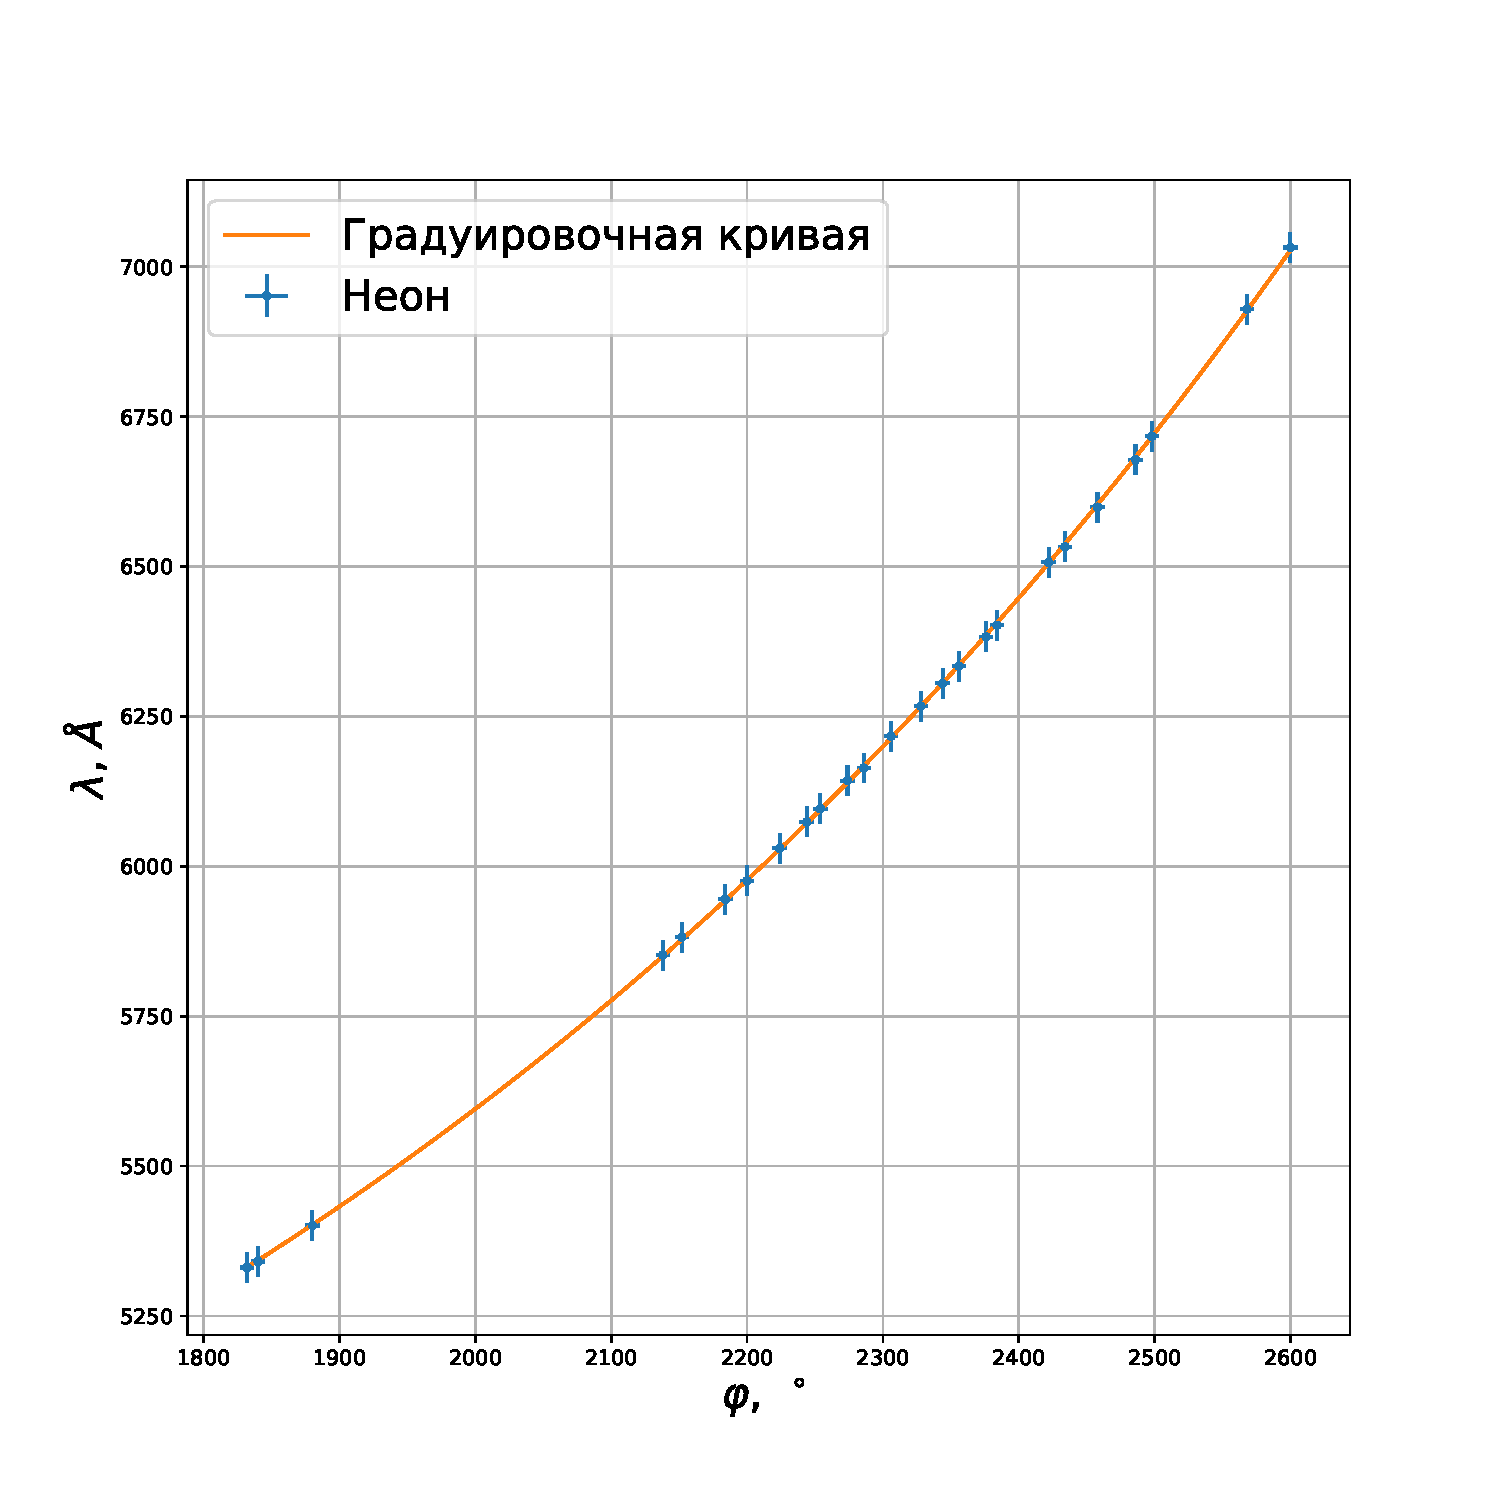
\includegraphics[scale = 0.35]{calib}
    \centering
    \caption{Калибровочный график}
    \label{img:calib}
\end{figure}

\begin{table}[H]
    \centering
    \begin{tabular}{|c|c|c|c|c|c|c|c|c|}
        \hline
        $I$, ед. & 0.282 & 0.336 & 0.381 & 0.415 & 0.44 & 0.458 & 0.475 & 0.488\\ \hline
        $U$, В   & 0.005 & 0.102 & 0.198 & 0.3 & 0.401 & 0.499 & 0.598 & 0.699
        \\ \hline
    \end{tabular}
    \\~\\
    \begin{tabular}{|c|c|c|c|c|c|c|c|c|}
        \hline
        $I$, ед. & 0.498 & 0.507 & 0.514 & 0.521 & 0.528 & 0.533 & 0.538 & 0.544\\ \hline
        $U$, В   & 0.802 & 0.905 & 1 & 1.101 & 1.198 & 1.302 & 1.399 & 1.504
        \\ \hline
    \end{tabular}
    \\~\\
    \begin{tabular}{|c|c|c|c|c|c|c|c|c|}
        \hline
        $I$, ед. & 0.548 & 0.552 & 0.556 & 0.56 & 0.563 & 0.566 & 0.57 & 0.578\\ \hline
        $U$, В   & 1.608 & 1.705 & 1.805 & 1.907 & 2 & 2.101 & 2.247 & 2.502
        \\ \hline
    \end{tabular}
    \\~\\
    \begin{tabular}{|c|c|c|c|c|c|c|c|c|}
        \hline
        $I$, ед. & 0.585 & 0.591 & 0.597 & 0.602 & 0.606 & 0.61 & 0.618 & 0.625\\ \hline
        $U$, В   & 2.751 & 3 & 3.249 & 3.509 & 3.749 & 4.003 & 4.502 & 4.994
        \\ \hline
    \end{tabular}
    \\~\\
    \begin{tabular}{|c|c|c|c|c|c|c|c|c|}
        \hline
        $I$, ед. & 0.631 & 0.637 & 0.641 & 0.644 & 0.128 & 0.037 & -0.02 & -0.036\\ \hline
        $U$, В   & 5.5 & 6.006 & 6.511 & 6.775 & -0.203 & -0.405 & -0.6 & -0.808
        \\ \hline
    \end{tabular}
    \\~\\
    \begin{tabular}{|c|c|c|c|c|c|c|c|}
        \hline
        $I$, ед. & -0.04 & -0.04 & -0.04 & 0.224 & 0.104 & 0.013 & -0.023\\ \hline
        $U$, В   & -0.994 & -1.204 & -1.406 & -0.1 & -0.294 & -0.506 & -0.695
        \\ \hline
    \end{tabular}
    \caption {$\phi = 1880$, $\lambda = 5402 \AA$}
\end{table}

\begin{table}[H]
    \centering
    \begin{tabular}{|c|c|c|c|c|c|c|}
        \hline
        $I$, ед. & 0.328 & 0.204 & 0.098 & 0.049 & 0.036 & 0.034\\ \hline
        $U$, В   & -0.045 & -0.217 & -0.408 & -0.598 & -0.795 & -0.998
        \\ \hline
    \end{tabular}
    \\~\\
    \begin{tabular}{|c|c|c|c|c|c|}
        \hline
        $I$, ед. & 0.33 & 0.436 & 0.476 & 0.504 & 0.521\\ \hline
        $U$, В   & -1.199 & 0.206 & 0.397 & 0.615 & 0.802
        \\ \hline
    \end{tabular}
    \caption {$\phi = 2050 \AA$, $\lambda = 5684 \AA$}
\end{table}

\begin{table}[H]
    \centering
    \begin{tabular}{|c|c|c|c|c|c|}
        \hline
        $I$, ед. & 0.334 & 0.431 & 0.479 & 0.506 & 0.526\\ \hline
        $U$, В   & 0.005 & 0.204 & 0.408 & 0.602 & 0.793
        \\ \hline
    \end{tabular}
    \\~\\
    \begin{tabular}{|c|c|c|c|c|c|}
        \hline
        $I$, ед. & 0.18 & 0.077 & 0.038 & 0.03 & 0.029\\ \hline
        $U$, В   & -0.2 & -0.396 & -0.594 & -0.803 & -0.983
        \\ \hline
    \end{tabular}
    \caption {$\phi = 2170$, $\lambda = 5915 \AA$}
\end{table}

\begin{table}[H]
    \centering
    \begin{tabular}{|c|c|c|c|c|c|c|}
        \hline
        $I$, ед. & 0.272 & 0.18 & 0.093 & 0.045 & 0.032 & 0.03\\ \hline
        $U$, В   & -0.026 & -0.147 & -0.292 & -0.456 & -0.603 & -0.808
        \\ \hline
    \end{tabular}
    \\~\\
    \begin{tabular}{|c|c|c|c|c|c|}
        \hline
        $I$, ед. & 0.385 & 0.444 & 0.481 & 0.505 & 0.529\\ \hline
        $U$, В   & 0.148 & 0.3 & 0.454 & 0.602 & 0.802
        \\ \hline
    \end{tabular}
    \caption {$\phi = 2300$, $\lambda = 6200 \AA$}
\end{table}

\begin{table}[H]
    \centering
    \begin{tabular}{|c|c|c|c|c|c|c|}
        \hline
        $I$, ед. & 0.23 & 0.338 & 0.417 & 0.459 & 0.492 & 0.519\\ \hline
        $U$, В   & 0.006 & 0.159 & 0.31 & 0.448 & 0.608 & 0.791
        \\ \hline
    \end{tabular}
    \\~\\
    \begin{tabular}{|c|c|c|c|c|c|}
        \hline
        $I$, ед. & 0.137 & 0.061 & 0.036 & 0.032 & 0.032\\ \hline
        $U$, В   & -0.138 & -0.297 & -0.451 & -0.6 & -0.809
        \\ \hline
    \end{tabular}
    \caption {$\phi = 2420$, $\lambda = 6500 \AA$}
\end{table}

\begin{table}[H]
    \centering
    \begin{tabular}{|c|c|c|c|c|c|c|}
        \hline
        $I$, ед. & 0.174 & 0.1 & 0.049 & 0.037 & 0.035 & 0.035\\ \hline
        $U$, В   & -0.022 & -0.15 & -0.294 & -0.435 & -0.594 & -0.797
        \\ \hline
    \end{tabular}
    \\~\\
    \begin{tabular}{|c|c|c|c|c|c|}
        \hline
        $I$, ед. & 0.274 & 0.367 & 0.429 & 0.474 & 0.51\\ \hline
        $U$, В   & 0.129 & 0.283 & 0.43 & 0.596 & 0.801
        \\ \hline
    \end{tabular}
    \caption {$\phi = 2500$, $\lambda = 6722 \AA$}
\end{table}

\begin{table}[H]
    \centering
    \begin{tabular}{|c|c|c|c|c|c|c|}
        \hline
        $I$, ед. & 0.129 & 0.194 & 0.293 & 0.366 & 0.428 & 0.479\\ \hline
        $U$, В   & 0.005 & 0.121 & 0.303 & 0.445 & 0.602 & 0.803
        \\ \hline
    \end{tabular}
    \\~\\
    \begin{tabular}{|c|c|c|c|c|c|}
        \hline
        $I$, ед. & 0.511 & 0.068 & 0.043 & 0.04 & 0.04\\ \hline
        $U$, В   & 0.994 & -0.138 & -0.284 & -0.442 & -0.607
        \\ \hline
    \end{tabular}
    \caption {$\phi = 2600$, $\lambda = 7027 \AA$}
\end{table}

\begin{figure}[H]
    \centering
    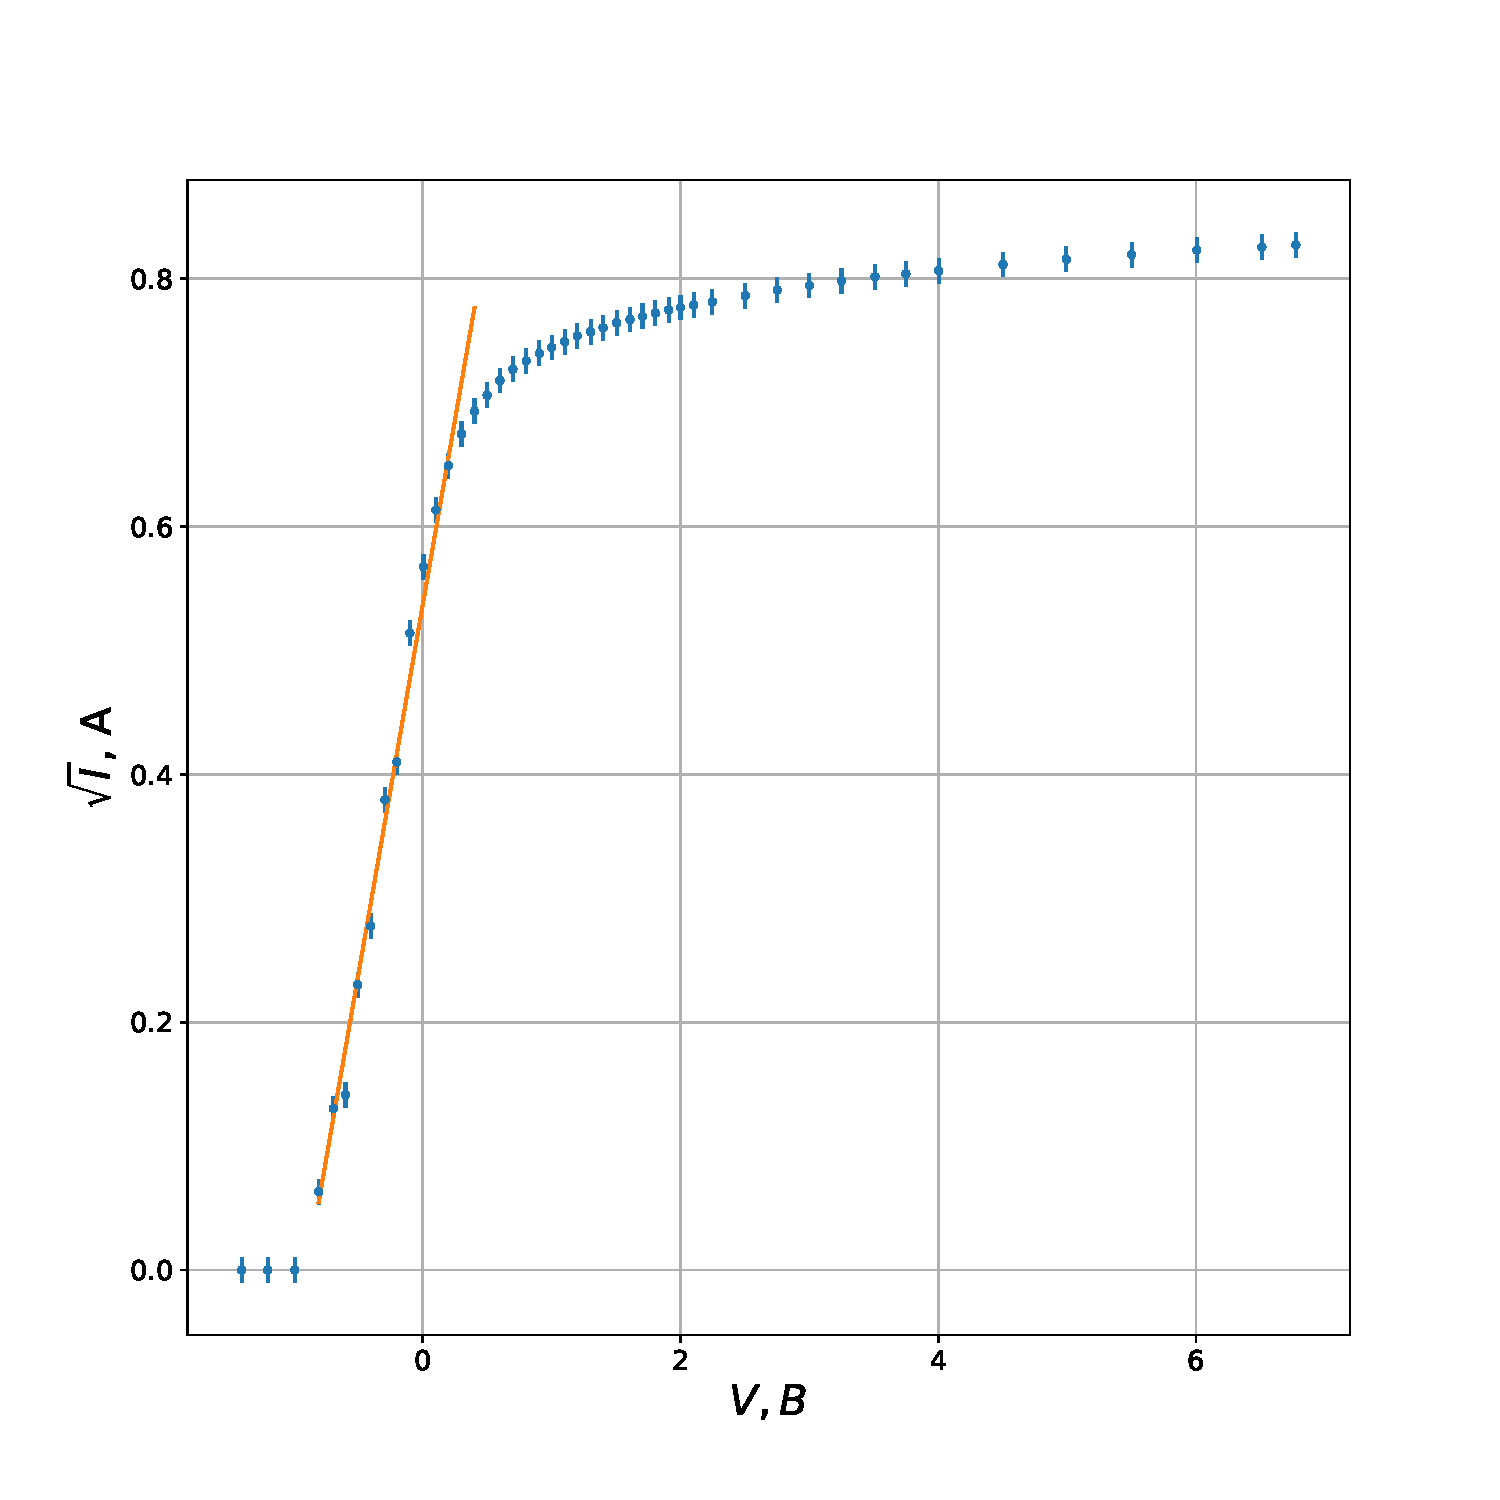
\includegraphics[scale=0.5]{1880}
    \caption {$\phi = 1880$, $\lambda = 5402 \AA$}
\end{figure}

\begin{figure}[H]
    \centering
    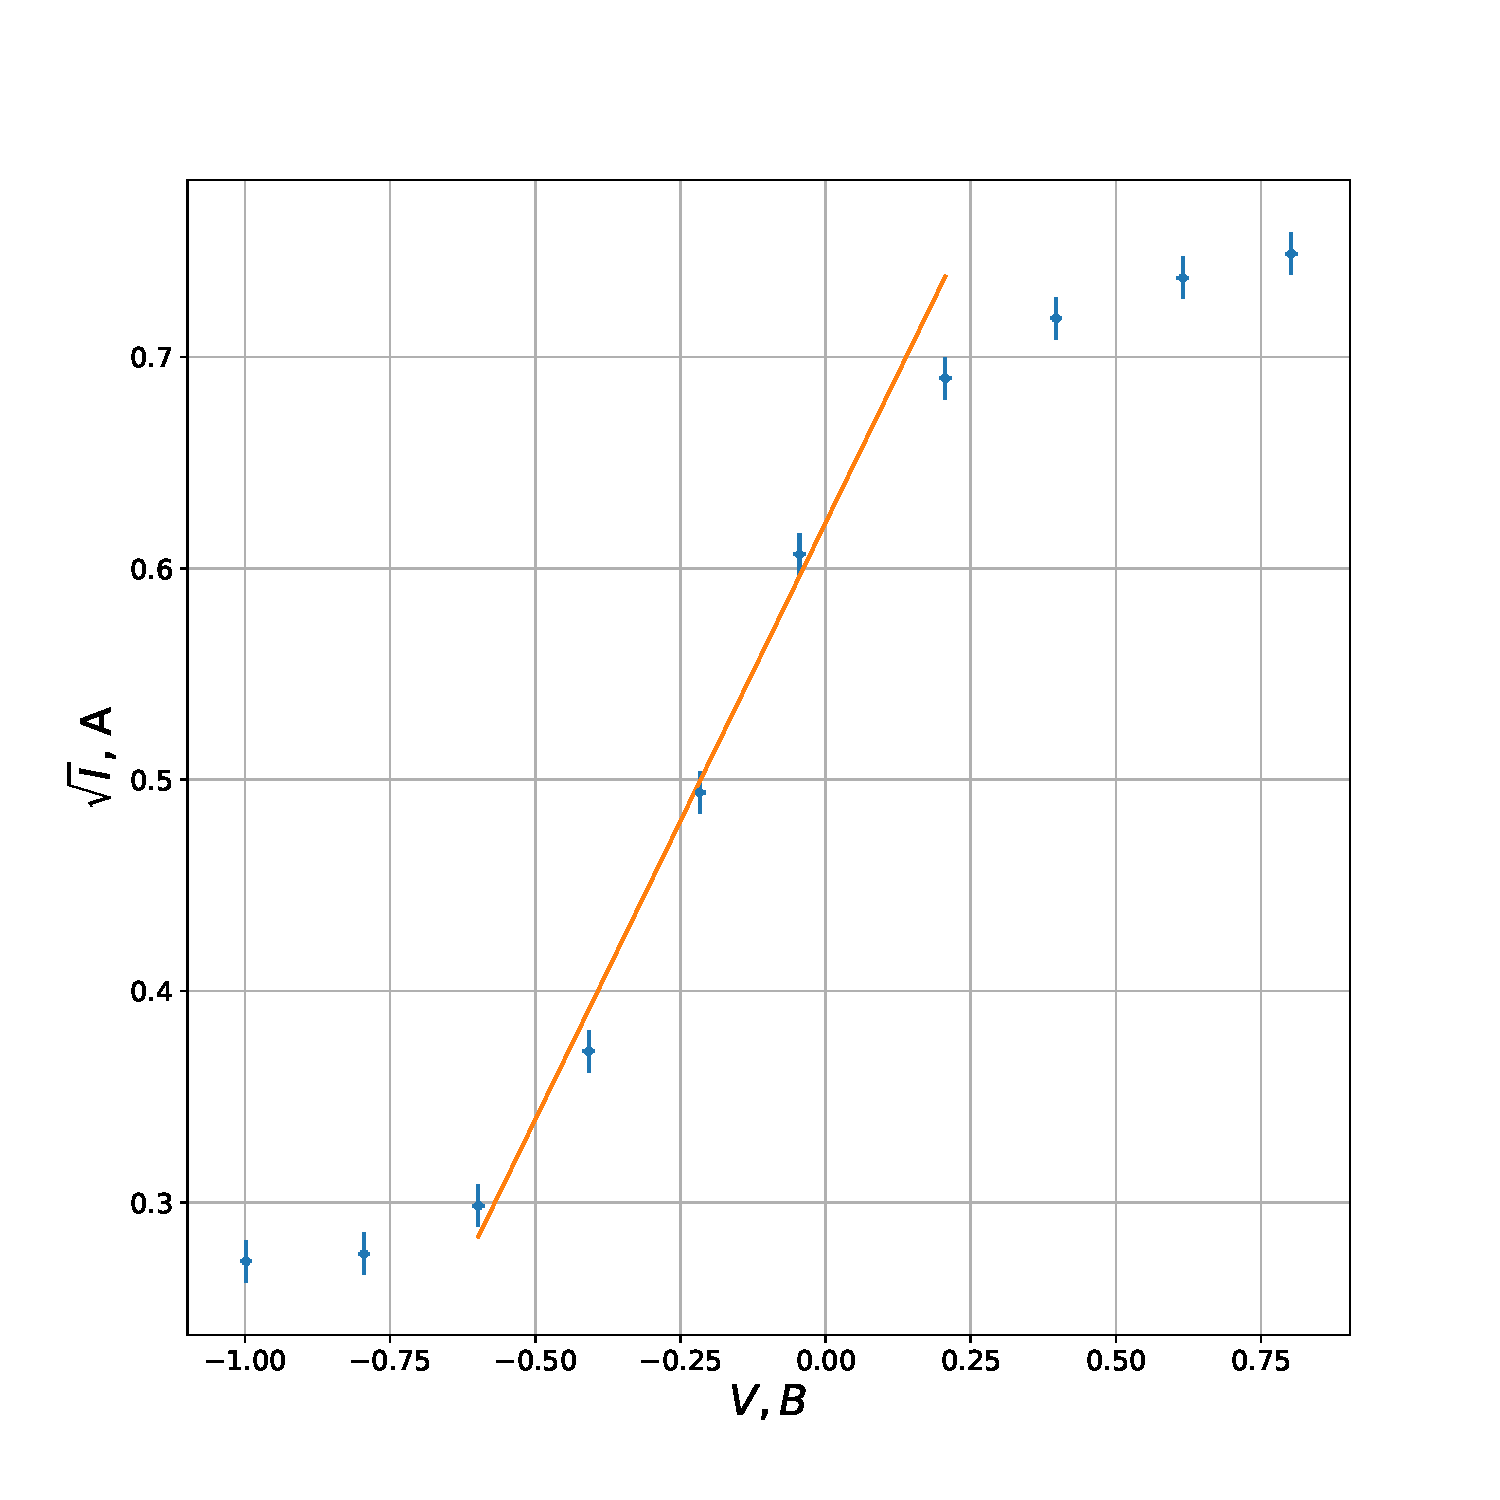
\includegraphics[scale=0.5]{2050}
    \caption {$\phi = 2050 \AA$, $\lambda = 5684 \AA$}
\end{figure}

\begin{figure}[H]
    \centering
    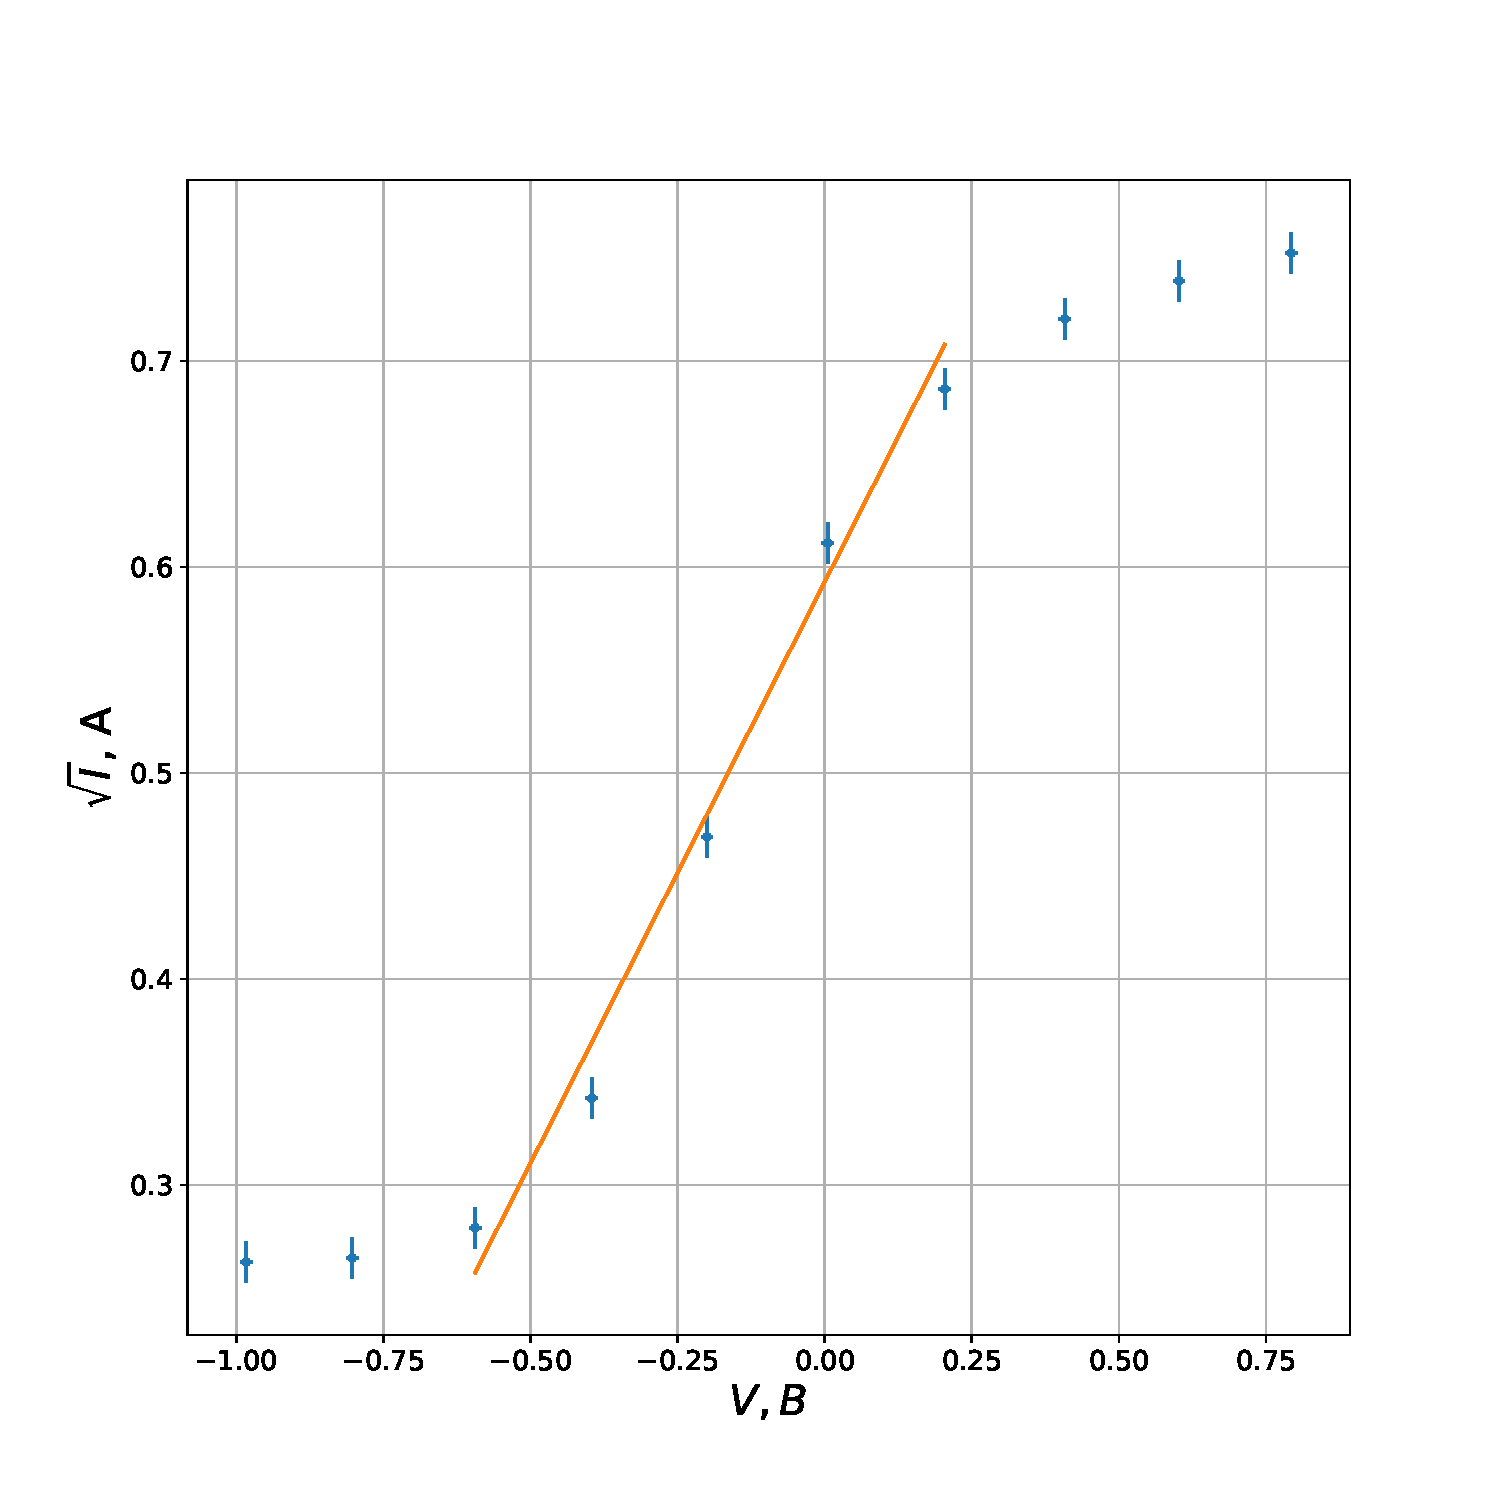
\includegraphics[scale=0.5]{2170}
    \caption {$\phi = 2170$, $\lambda = 5915 \AA$}
\end{figure}

\begin{figure}[H]
    \centering
    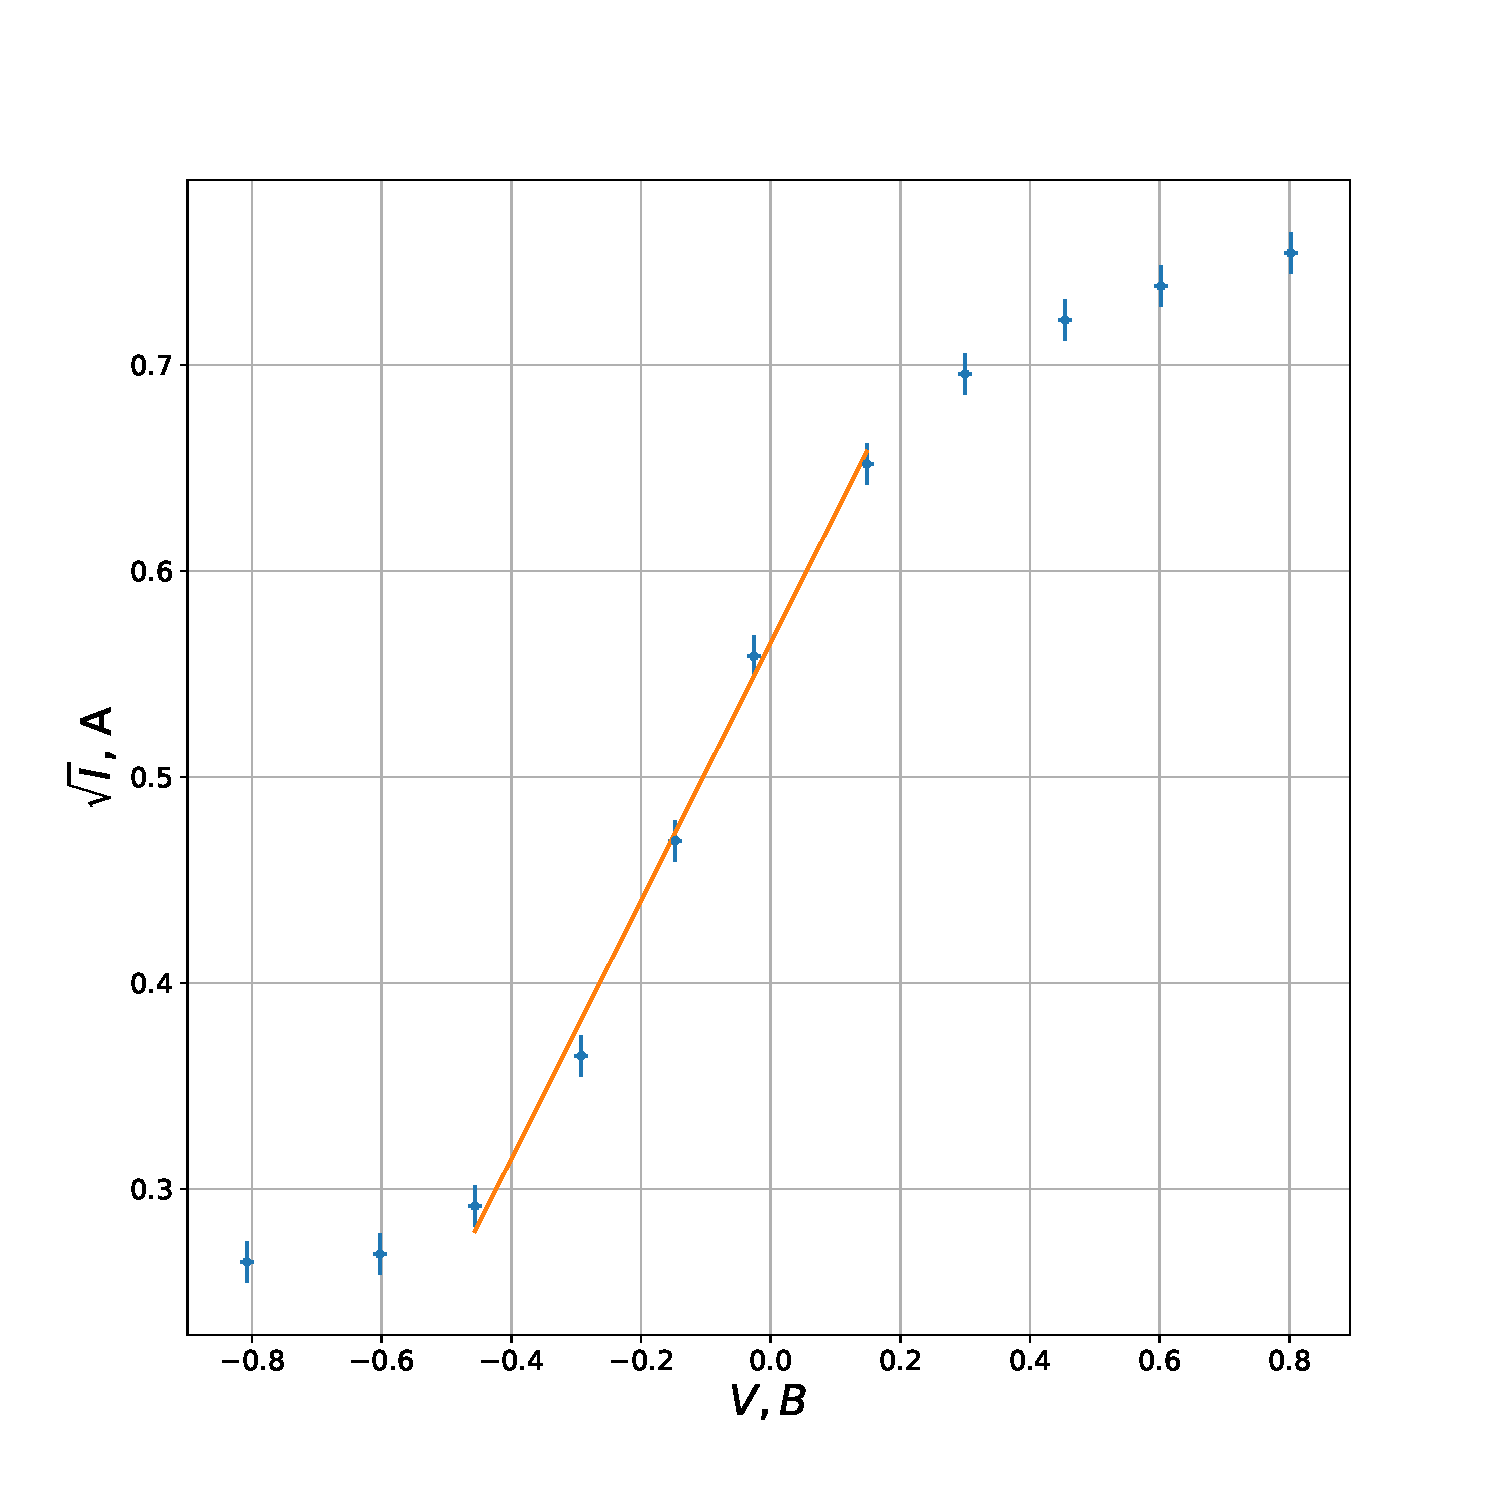
\includegraphics[scale=0.5]{2300}
    \caption {$\phi = 2300$, $\lambda = 6200 \AA$}
\end{figure}

\begin{figure}[H]
    \centering
    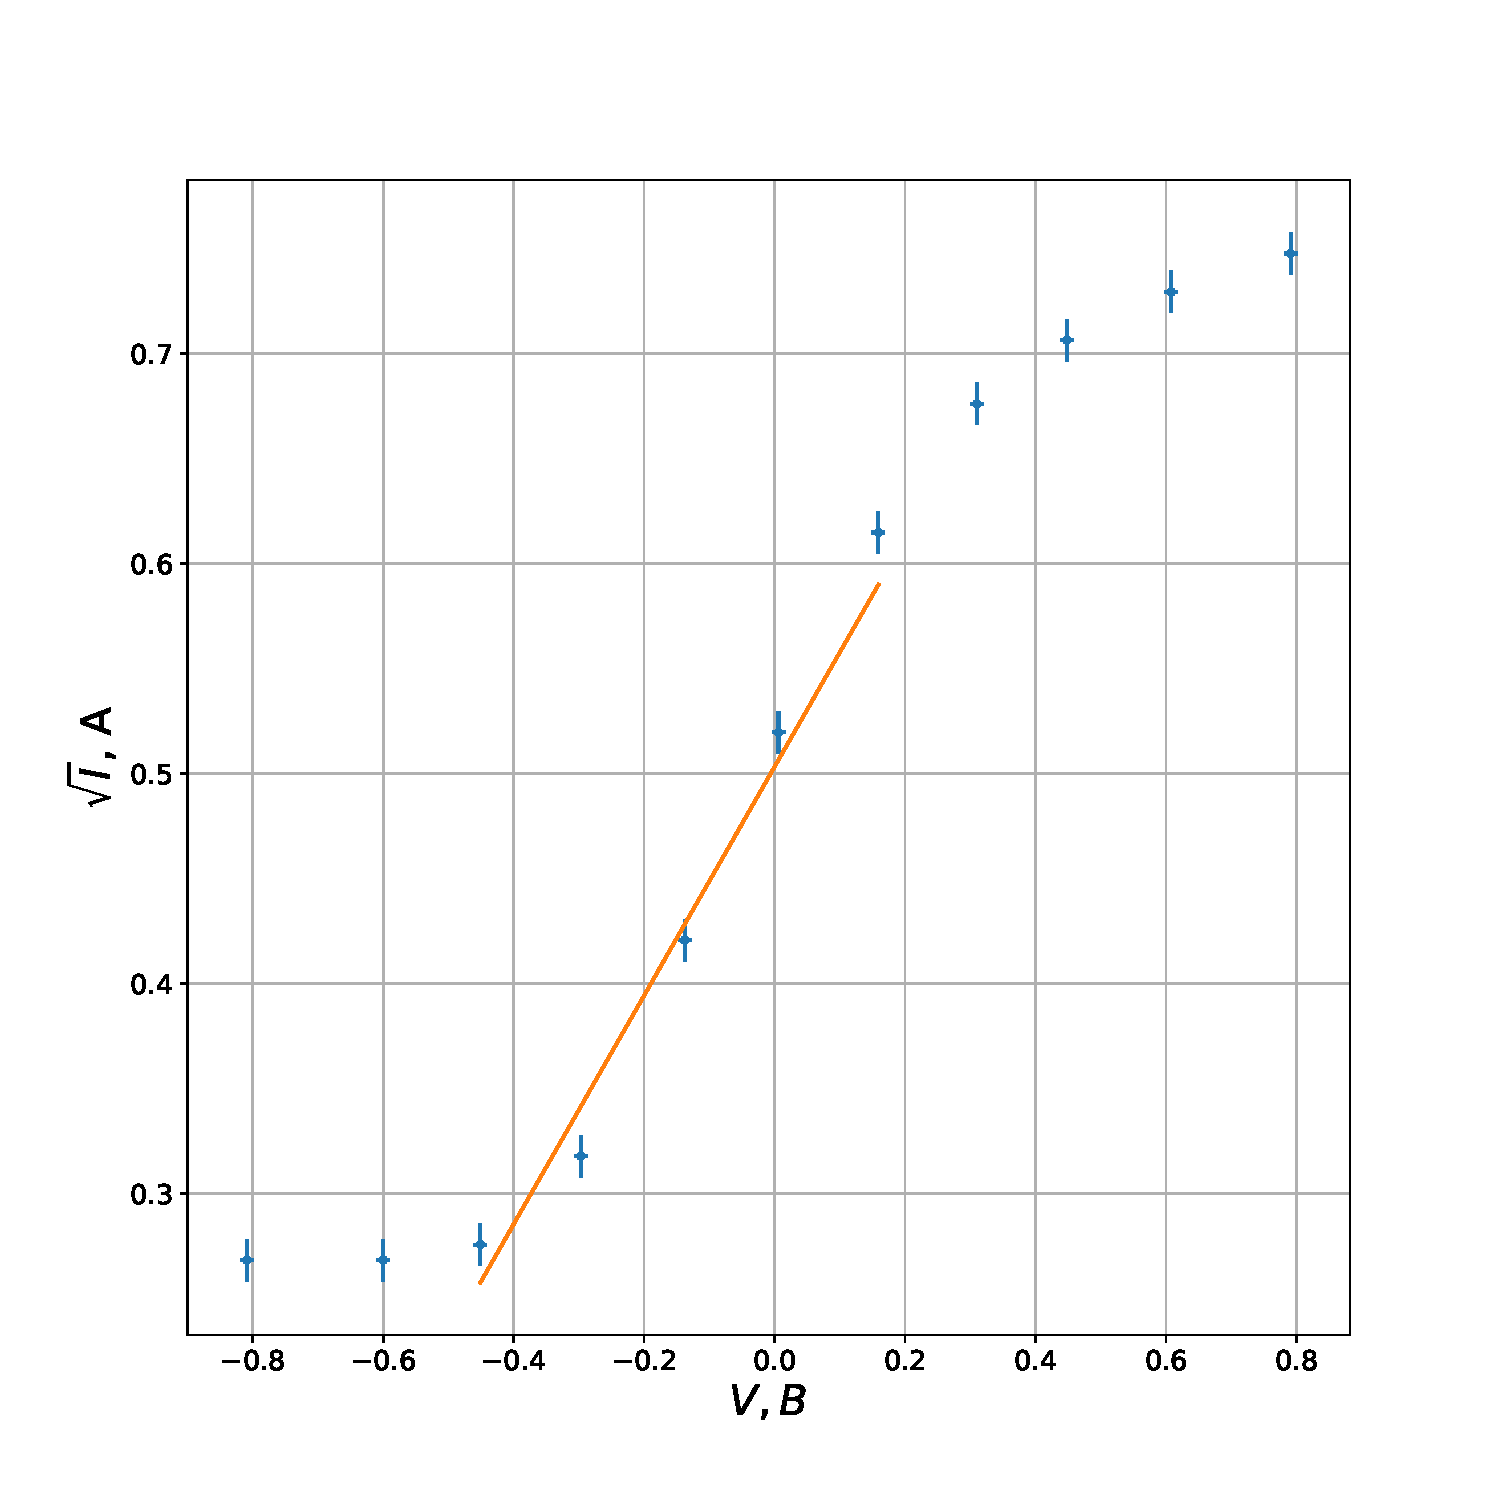
\includegraphics[scale=0.5]{2420}
    \caption {$\phi = 2420$, $\lambda = 6500 \AA$}
\end{figure}

\begin{figure}[H]
    \centering
    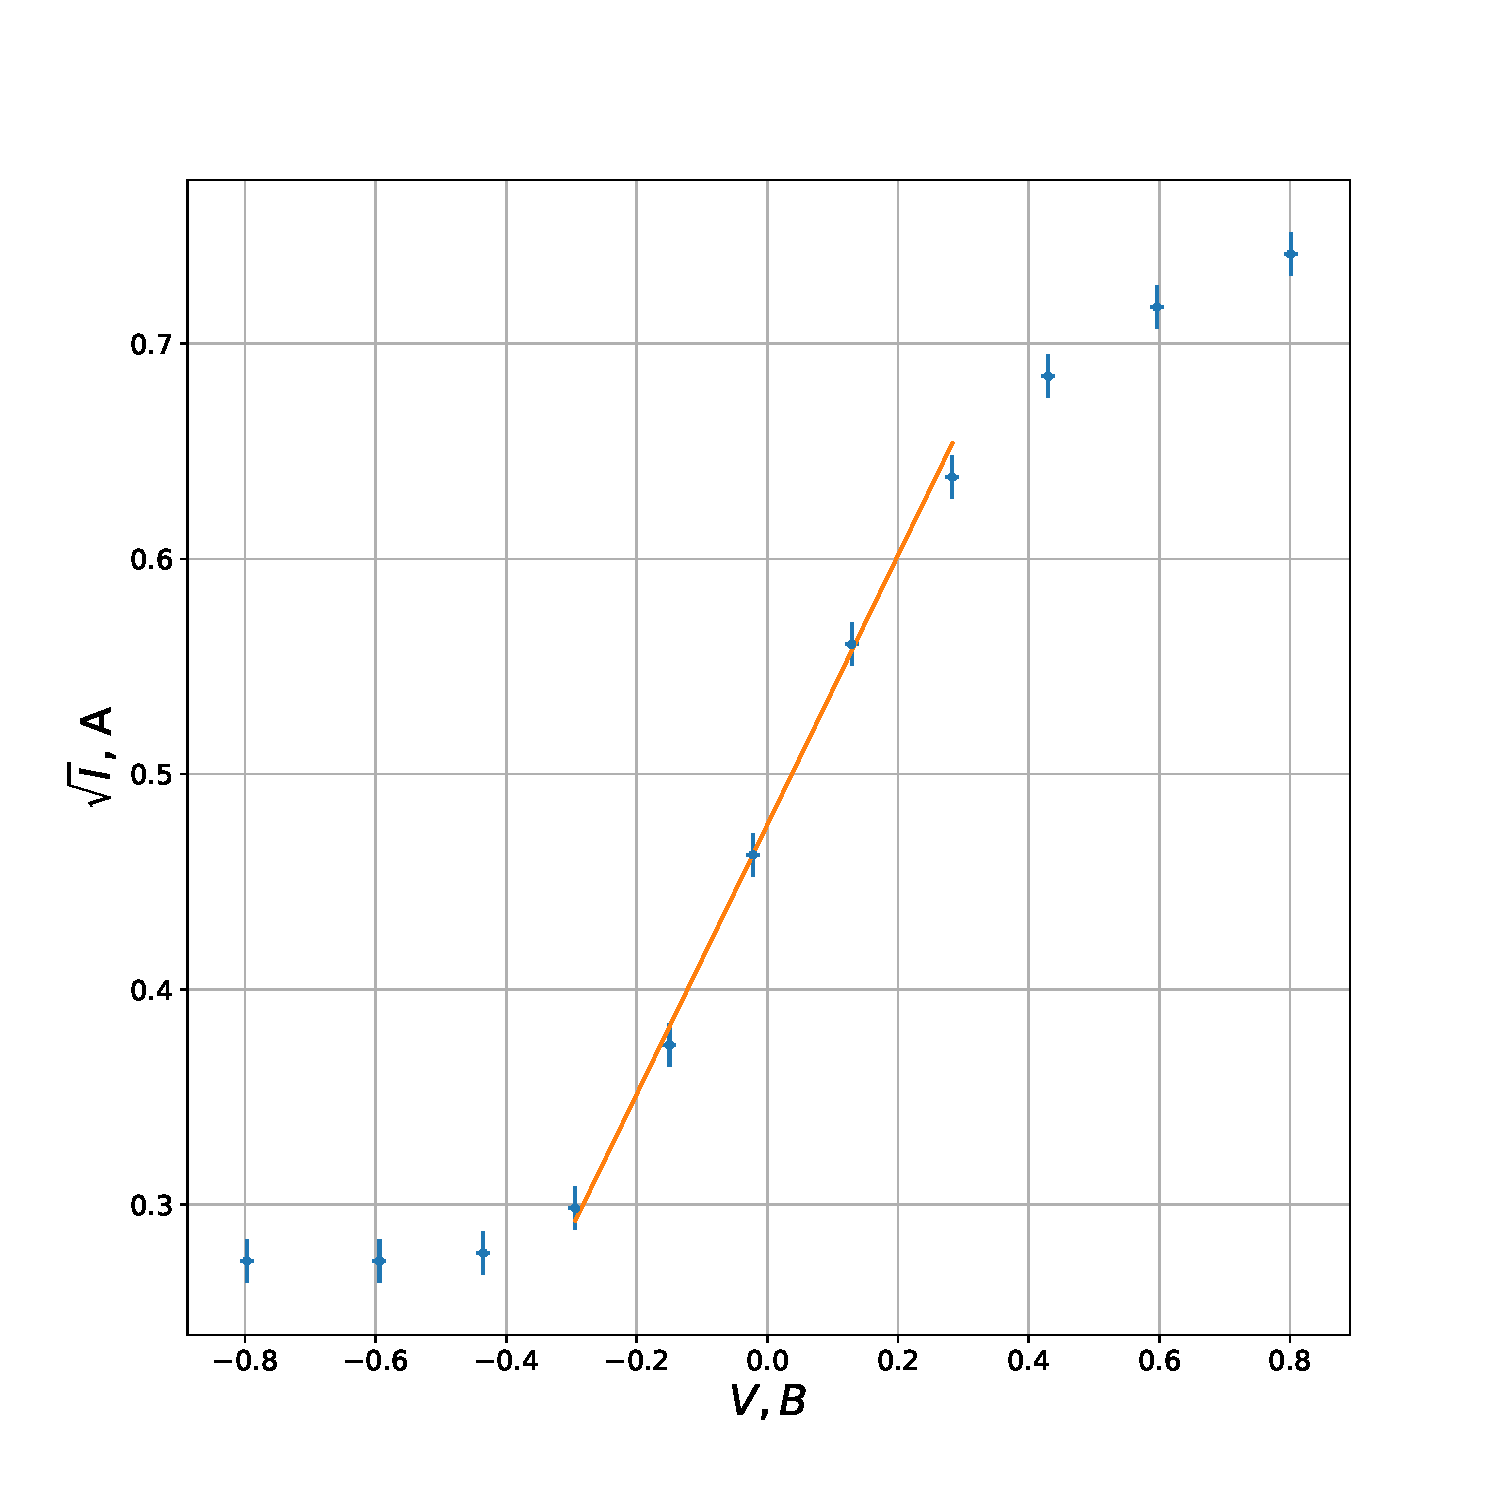
\includegraphics[scale=0.5]{2500}
    \caption {$\phi = 2500$, $\lambda = 6722 \AA$}
\end{figure}

\begin{figure}[H]
    \centering
    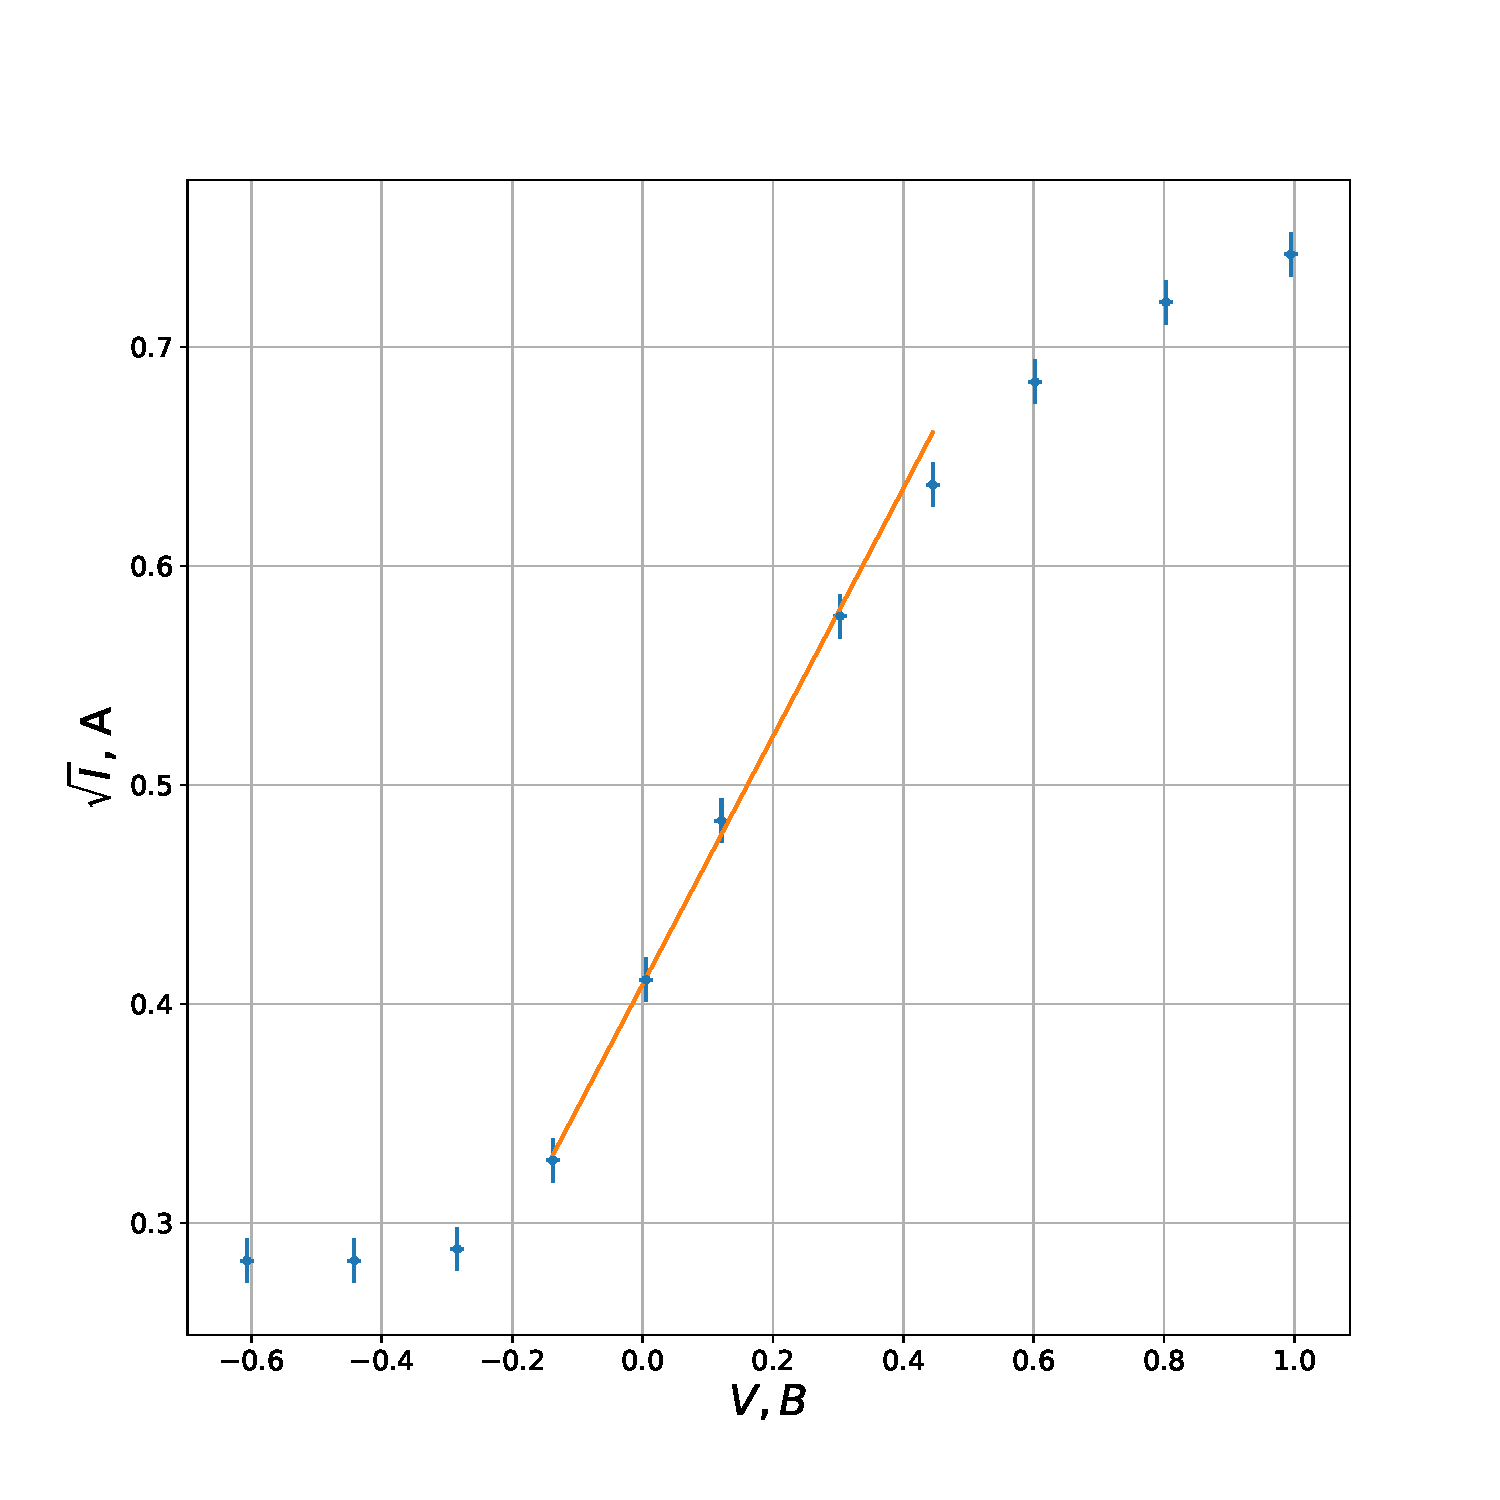
\includegraphics[scale=0.5]{2600}
    \caption {$\phi = 2600$, $\lambda = 7027 \AA$}
\end{figure}

\begin{table}[H]
    \centering
    \begin{tabular}{|c|c|c|c|c|c|c|c|c|}
        \hline
        $\phi, ~^\circ$ & $\lambda, ~\AA$ & $\omega, ~10^{15}~\frac{1}{с}$ & $k$ & $\sigma_k$ & $b$ & $\sigma_b$ & $V_0$ & $\sigma_{V_0}$ \\ \hline
        1880 & 5402 & 3.489 & 0.576 & 0.018 & 0.535 & 0.007 & 0.93 & 0.03\\ \hline
        2050 & 5684 & 3.316 & 0.565 & 0.032 & 0.621 & 0.006 & 1.10 & 0.06\\ \hline
        2170 & 5915 & 3.187 & 0.586 & 0.035 & 0.583 & 0.007 & 0.99 & 0.06\\ \hline
        2300 & 6200 & 3.040 & 0.618 & 0.023 & 0.562 & 0.004 & 0.91 & 0.03\\ \hline
        2420 & 6500 & 2.900 & 0.654 & 0.005 & 0.512 & 0.001 & 0.78 & 0.01\\ \hline
        2500 & 6722 & 2.804 & 0.625 & 0.017 & 0.476 & 0.002 & 0.76 & 0.02\\ \hline
        2600 & 7027 & 2.682 & 0.566 & 0.011 & 0.408 & 0.001 & 0.72 & 0.01
        \\ \hline
    \end{tabular}
\end{table}

\begin{figure}[H]
    \centering
    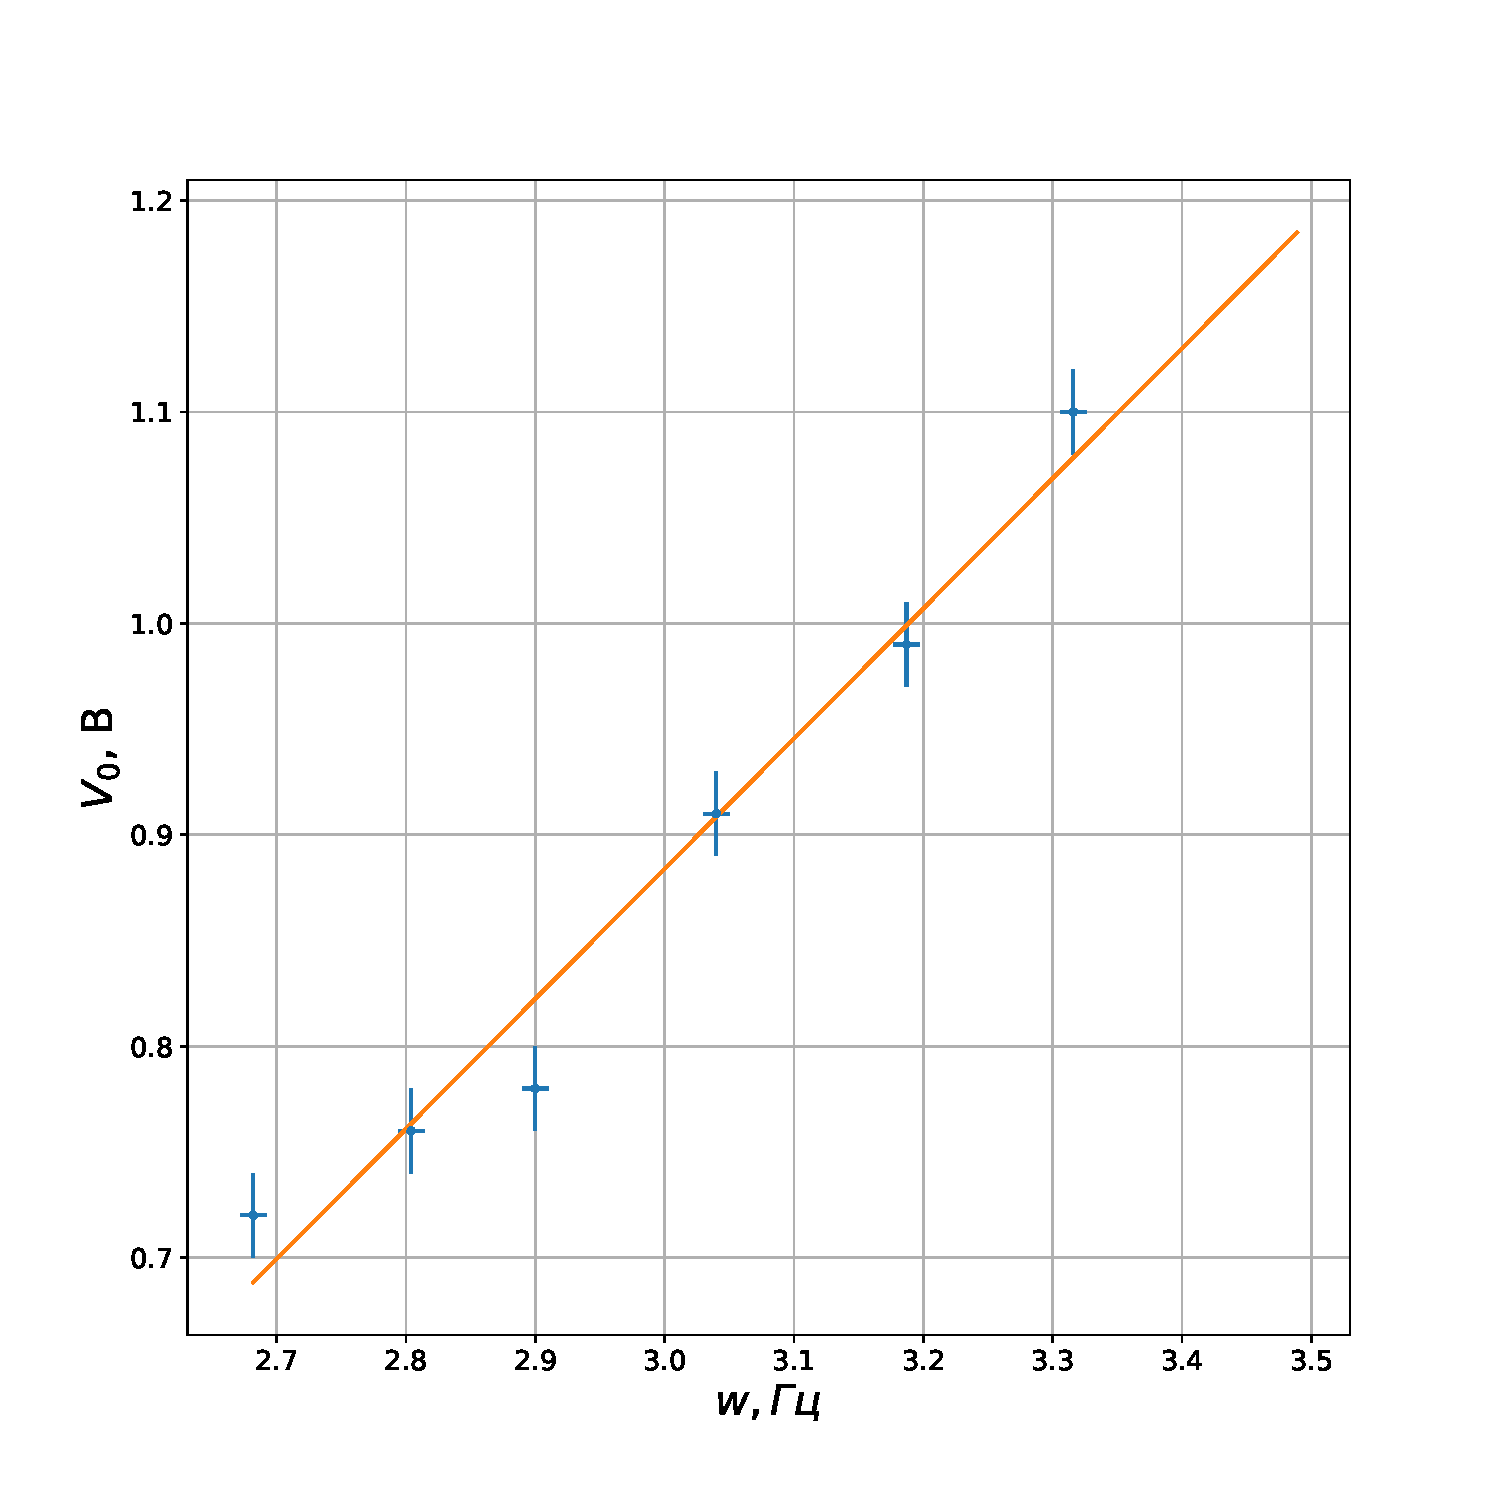
\includegraphics[scale=0.5]{V0}
    \caption {$V_0 (\omega)$}
\end{figure}

 
	

\end{document}
